\section{Experiments}
\label{sec:experiments}

Every number below comes from a protocol frozen with its criteria, thresholds and
predeclared outcomes written down \emph{before} the run that tests them; each
protocol's SHA-256 is recorded on disk at freeze time and amendments are appended,
never edited in. Where a criterion failed we report the failure under its own
name. Two amendments in our record retract earlier claims of \emph{ours}, and we
cite them rather than quietly dropping them.

\subsection{Stream, model, and budget}
\label{sec:setup-exp}

\paragraph{Stream.}
The $15$-task Order-4 sequence: MNLI, CB, WiC, COPA, QQP, BoolQA, RTE, IMDB,
Yelp, Amazon, SST-2, DBpedia, AGNews, MultiRC, Yahoo. Its scope structure is the
table in Section~\ref{sec:setup}: four multi-task scopes plus five singletons.
Tasks are presented as prompts with an explicit option list, so a task-free rule
may read the option list but never a task index.

\paragraph{Model and budget.}
T5-large with LoRA rank $8$ on $q/v$: $2{,}359{,}296$ trainable scalars, identical
in every arm and verified per arm at run time. $400$ examples per class per task,
$3$ epochs, effective batch $64$, giving $813$ gradient steps per seed. Three
seeds throughout.

\paragraph{Splits.}
Each task is partitioned into disjoint \texttt{update} (training),
\texttt{risk} ($64$/class) and \texttt{audit} ($64$/class) sets, all carved from
the training file. Offsets are \emph{fit} on \texttt{risk} and \emph{scored} on
\texttt{audit}; \texttt{risk} is never reported as a level. The official test
files are never opened at any point in this paper. Yelp and Amazon are excluded
from scored means because their five-way verbalizers share first sub-word pieces
(\texttt{very negative} / \texttt{very positive}), and CB because its rarest class
has $16$ examples, below the $40$ that a $64$/class risk-plus-audit split needs.
Twelve of fifteen tasks remain scorable.

\paragraph{Statistics.}
All intervals are cluster bootstrap with \emph{tasks as clusters}, $10{,}000$
draws. Tasks are the clusters because the same task measured at different stages
shares its data and its model state, so resampling examples would understate
variance. Point estimates are medians unless stated otherwise.

\paragraph{Unconditional training gate.}
Median post-training $R^{\mathrm{raw}}>0.60$, reported for every arm whatever its
value. Below the gate an arm has not learned the stream and nothing about its
forgetting is interpretable. Every arm below passes it.

\subsection{The identification gap is real and the scope index closes it}
\label{sec:gap-real}

We first ask whether $\Delta^{\mathrm{id}}$ of \eqref{eq:delta-id} exists at a size
worth a method, using no continual-learning intervention at all (the
\texttt{none} arm).

Median $\Delta^{\mathrm{id}}$ against a single global offset is
$\mathbf{3.13}$~pp. Median $\Delta^{\mathrm{id}}$ against a per-scope offset is
$\mathbf{0.0000}$. The identification gap is therefore not a residue of the argmax
being hard to hit: it is almost entirely explained by \emph{which scope the query
is in}, and a rule that reads the option list --- needing no task index --- closes
it at the median.

Two checks accompany that pair. Proposition~\ref{prop:disjoint} predicts exactly
zero gap on singleton scopes; across $87$ singleton observations we find $0$
violations, worst absolute deviation $0.0$, and the check passes with $0$
violations in every arm below. And the ladder is monotone in codebook size $m$,
Spearman $\rho(q_m,\text{worst loss})=+0.646$ over $513$ points.

The rest of the ladder does \emph{not} pay. Moving from one offset per scope to an
$m$-centre codebook per scope, selected by a task-free prototype router, buys a
median of exactly $\mathbf{0.0000}$ across $11$ tasks; a post-hoc restriction to
the $7$ tasks in multi-task scopes also fails, with an interval containing zero.
This was a preregistered criterion and we report it as failed, not as a tie. The
reading is that on this stream the useful identification budget is one offset per
scope; finer codebooks are unnecessary rather than harmful.

\paragraph{The offset ladder, measured.}
Table~\ref{tab:offset-ladder} gives the ladder on the \texttt{none} arm, three
seeds, mean over the $12$ scorable tasks.
\begin{table}[t]
\centering
\small
\caption{The identification ladder on the \texttt{none} arm (three seeds, mean over
the $12$ scorable tasks). Per-scope over global is $+1.51$~pp, CI $[+0.43,+2.74]$;
the oracle task index adds only $+0.02$~pp pooled, and a finer codebook adds
nothing.}
\label{tab:offset-ladder}
\begin{tabular}{lcl}
\toprule
inference rule & mean accuracy & requires \\
\midrule
no offset                       & $0.7016$ & --- \\
one global offset               & $0.7077$ & nothing \\
one offset per scope            & $0.7227$ & the option list \\
$m=4$ codebook per scope        & $0.7227$ & the option list \\
one offset per task (oracle)    & $0.7229$ & \emph{the task index} \\
\bottomrule
\end{tabular}
\end{table}
Per-scope over global is $\mathbf{+1.51}$~pp, CI $[+0.43,+2.74]$, excluding zero.
On multi-task scopes oracle over per-scope is $+1.10$~pp, CI $[+0.40,+1.83]$; the
pooled figure across all scopes is $+0.02$~pp, CI $[-1.00,+1.00]$. We previously
read that pooled figure as \emph{the task index buys nothing beyond the scope
index}, and used it as the empirical licence for treating rung 3 of
Section~\ref{sec:ladder} as the deployable target. Disclosure~(iii) below
withdraws that reading: the pooled $+0.02$ averages over rows where our
implementation forces the two rungs to be \emph{identical by construction}, so it
cannot license anything. The licence for
rung 3 now rests on the cost argument of Section~\ref{sec:enumeration} alone,
not on a measured equality.

Three disclosures that bound the claim; (i) and (ii) were frozen before we
measured them, (iii) was found after scoring and is reported with that status. (i)
Restricted to multi-task scopes alone, per-scope over global is $+1.17$~pp with CI
$[-0.09,+2.91]$ --- not significant; most of the $+1.51$~pp arises on singleton
scopes, where by Proposition~\ref{prop:disjoint} the scope \emph{is} the task.
(ii) The per-scope row above is refit at each stage from the \texttt{risk} logits
of \emph{all seen tasks}. It re-reads old data, so it is a rehearsal ceiling and
not a deployable method. Section~\ref{sec:sso} exists because of that.
(iii) \textbf{The oracle$-$per-scope comparison is not measurable on singleton
scopes in our implementation.} On a scope holding one task, the code assigns that
task's own fitted offset to the scope rather than re-running the shared fit
(\texttt{run\_qoc.py}, \texttt{scoped\_shared\_offsets}). That substitution is
sound as an \emph{estimand} --- with one task in the pool, minimising worst-task
loss and maximising that task's own objective have the same optimum, which is why
the per-scope-over-global $+1.51$~pp is unaffected --- but it makes
$R^{\mathrm{orc}}-R^{\mathrm{shr}}_{\mathrm{scope}}$ exactly zero on those rows
as an identity, not as a finding. Empirically those rows are $783$ of $2511$ and
$100\%$ of them are exactly zero. Restricted to multi-task scopes, where the
comparison is live, the gap is $+1.10$~pp with cluster-bootstrap CI
$[+0.40,+1.83]$ over $7$ task clusters, positive in $27$ of $27$ runs
(sign test $p=7.5\times10^{-9}$), and $+2.34$~pp CI $[+0.71,+4.12]$ if restricted
further to the final stage. So the task index \emph{does} buy something beyond the
scope index wherever we can actually measure it. This recomputation uses the $27$
runs held locally, not the converged run that produced the $+0.02$ above, so it is
reported as a separate measurement rather than as a restatement of that row.

\subsection{Three parameter-space interventions do not touch this term}
\label{sec:three-anchors}

If the identification gap is a property of the output layer under shared
verbalizers, interventions that spend the parameter budget differently should
leave it in place. We tested three, each with its own frozen protocol, its own
pre-registered $\lambda$ gate on a held-out split, and its own predeclared
outcomes. All three are reported as they landed.

\paragraph{(a) Orthogonality between task subspaces (O-LoRA form).}
\label{sec:2l}
Penalty $\lambda\sum_{t<g}\lVert \bA_g\bA_t^\top\rVert_F^2$ with previous $\bA_t$
detached; $\lambda$ selected before the confirmatory run from $\{0.1,0.5,1.0\}$ by
a gate on the \texttt{update} split, which chose $\lambda=0.5$ at an interior
optimum. The criterion that had to pass first was not additivity but
\emph{efficacy}: median repair of raw retention in the stratum where forgetting
exceeds $8$~pp. It failed, at both $\lambda$: $+0.50$~pp, CI $[-1.56,+4.69]$ at
$\lambda=0.5$ and $+0.00$~pp, CI $[-2.95,+7.03]$ at $\lambda=1.0$, $n=34$ cells.
The protocol states that if efficacy fails the additivity readings are
uninterpretable, so we do not report them as evidence in either direction. The
near-zero median is a real cancellation, not inertness: BoolQA is repaired
$+6.58$~pp while MNLI --- the largest forgetting event in the stream at $24.5$~pp
--- is made \emph{worse} by $3.47$~pp, and RTE, with $15.7$~pp of forgetting, moves
$+0.13$~pp. This is our re-implementation of the regulariser inside our harness at
our budget; it is not a reproduction of the original authors' numbers and no
comparison against their published table is made or implied.

\paragraph{(b) Anchoring the verbalizer logits (VLA).}
A penalty pulling each task's verbalizer logits toward their post-training values,
$\lambda$ gated as above, which selected $\lambda_a=8.0$. Preregistered criterion 1
--- that the anchor improve task-agnostic accuracy --- \textbf{failed}:
$\mathbf{-4.78}$~pp, CI $[-7.36,-2.25]$. Accuracy fell from $0.7077$ to $0.6599$
while the training gate passed at $0.7188$. At the gate-selected $\lambda$ the
anchor is not inert; it is harmful.

The qualifier is load-bearing and we add it because our own secondary arm
contradicts the unqualified version. At $\lambda_a=0.5$, completed to three seeds,
criterion 1 also fails but from the other side: $+0.28$~pp, CI $[-1.24,+1.90]$ ---
no detectable effect rather than damage. That arm is not headline-eligible under the
protocol's own rule that only the gate-selected $\lambda$ may be quoted as the
result, and we do not promote it. But it means the honest claim is that VLA is
harmful \emph{at the strength the gate chose}, not that logit anchoring is harmful
as such. We also record that this arm read $-5.66$~pp on its first seed alone, and
that the $6$~pp effect vanished when the remaining two seeds landed.

\paragraph{(c) Gauge-fixed anchoring (GFA).}
VLA's failure has an obvious diagnosis: the anchored quantity is not
gauge-invariant, and a penalty that pins the unidentified part of the offset
wastes capacity fighting a symmetry. GFA anchors only the zero-mean projection
$P_0\bz_S$, which is gauge-invariant to machine precision by construction and by
test. Criterion 1 \textbf{failed harder}: $\mathbf{-6.29}$~pp, CI
$[-9.37,-3.16]$, accuracy $0.7077\to0.6448$.

\paragraph{What (c) tells us, which is more than that it failed.}
GFA came with a preregistered gauge check: if the damage is caused by the
non-invariance that GFA removes, then the fraction of GFA's damage repairable by a
free per-scope constant must fall below a $2$~pp tolerance. It did not. That
fraction is $\mathbf{1.042}$ for GFA against $1.059$ for VLA --- essentially all of
the damage remains gauge-shaped, at $6.55$~pp against the $2$~pp tolerance. A
gauge-invariant \emph{objective} did not produce a gauge-invariant
\emph{solution}: pinning $P_0\bz_S$ leaves $\mathrm{mean}(\bz_S)$ unpenalised, and
the shared adapter update moves it freely. Two further readings, both against us:
the largest irreparable loss lands on \emph{single-task} scopes ($-8.06$~pp raw,
$-3.49$~pp even after a per-scope offset), i.e.\ outside the penalty's own sum;
and the quantization radii $q_1,q_2$ both \emph{increased} ($+0.036$, $+0.009$),
the opposite of what the intervention was designed to do. We also record that
GFA's $6$-task $\lambda$ gate did not predict its $15$-task behaviour, and that
one claim we made in that amendment about a scope-class split ($+2.95$~pp on
multi-task scopes) was withdrawn in a later amendment once we bootstrapped it: CI
$[-5.54,+11.94]$, $n=7$, not significant, resting on two tasks against two of
opposite sign.

\paragraph{Summary of (a)--(c).}
Three interventions, three frozen protocols, $2.36$M trainable scalars each.
None improved task-agnostic accuracy; two actively reduced it; the one designed
from the correct symmetry argument did the most damage. The identification gap
survived all three, and the per-scope offset kept recovering $+1.51$~pp on top of
each. We take this as evidence that the gap is not a parameter-space object, and
we note the alternative reading --- that better parameter-space interventions
exist and we did not find them --- as the limitation it is.

\paragraph{A counterexample to our own geometric story, from our own runs.}
Proposition~\ref{prop:cheb} makes the Chebyshev radius $r_S$ the quantity that
governs the best shared offset, so the natural inference is that shrinking it
should raise the retained level. It does not, and we have a clean instance.
VLA's protocol pre-registered a criterion on exactly this: that $q_1$ and $q_2$
decrease. That criterion \textbf{passed} --- $q_1$ from $0.0761$ to $0.0616$ and
$q_2$ from $0.0284$ to $0.0158$ over the $8$ shared scopes, both directionally down
--- in the \emph{same run} whose accuracy criterion failed at $-4.78$~pp. We had
predicted the radii would not move, so this also falsifies a prediction of ours in
the direction that is inconvenient: the mechanism was right about its own quantity
and wrong about the consequence.

The lesson is a bound on the theory's reach, and it is the same bound the constant
$\kappa$ measures. A small $r_S$ is necessary for a shared offset to do well; it is
not sufficient for accuracy, because the map from logit distance to flipped
predictions can be arbitrarily flat --- Proposition~\ref{prop:no-free-lunch} in
Appendix~\ref{app:kappa-necessary} shows no assumption-free version of that step
exists, and our measured $\kappa\approx0.018$ says the map is nearly flat on this
benchmark. \textbf{Tightening $q_m$ therefore does not license an accuracy claim},
and no argument in this paper makes that inference. It is also why every
accuracy-space number we report is measured rather than derived from
\eqref{eq:cheb-acc}.

\subsection{Admissible rule 1: storing the offsets fails, and the reason is measurable}
\label{sec:sso}

The first of the two rules Section~\ref{sec:enumeration} admits stores the table.
At each task boundary, fit that task's optimum on its own \texttt{risk} split,
keep it, and at test time apply the Chebyshev centre of its scope's entries. No
task ID, no stored examples, no rehearsal, $33$ floats. We froze this as Phase-2P
with a primary criterion P1 (beat the single global offset) and five others, then
ran it on three seeds.

\textbf{It does not work, and it is worse than doing nothing.}
Table~\ref{tab:sso} gives the levels. SSO($m{=}1$) scores $0.6509$ against
$0.7016$ for applying no offset at all --- $5.08$~pp \emph{below} the floor --- and
$5.68$~pp below the global offset it was meant to beat, CI $[-8.41,-3.16]$. P3
shows the damage is not concentrated in an outlier: $11$ of $12$ tasks lose
individually, worst QQP at $-14.84$~pp. P4, which the protocol had already
predicted would fail, failed: a $4$-centre codebook adds $+0.52$~pp, CI
$[-0.46,+1.74]$.

\begin{table}[t]
\centering
\small
\caption{Phase-2P, mean over the $12$ scorable tasks at the final stage, three
seeds. Storing offsets is $5.08$~pp worse than storing nothing. The rehearsal
columns are ceilings, not rivals.}
\label{tab:sso}
\begin{tabular}{lcccccc}
\toprule
 & no offset & global & \textbf{SSO} $m{=}1$ & SSO $m{=}4$ & per-scope & per-task \\
 & $R^{\mathrm{raw}}$ & $R^{\mathrm{glob}}$ & \textbf{stored} & stored & refit & refit \\
\midrule
rehearsal-free & \checkmark & --- & \checkmark & \checkmark & --- & --- \\
accuracy & $0.7016$ & $0.7077$ & $\mathbf{0.6509}$ & $0.6561$ & $0.7227$ & $0.7229$ \\
\bottomrule
\end{tabular}
\end{table}

\paragraph{Singleton scopes isolate the cause.}
The interesting part is not that P1 failed but that the design lets us say why:
Table~\ref{tab:sso-singleton} splits the loss by scope size.

\begin{table}[t]
\centering
\small
\caption{Storing offsets (SSO $m{=}1$) minus the global offset, split by scope size,
three seeds. The loss persists on singleton scopes --- where the Chebyshev centre of
a one-element table \emph{is} that element, so there is no aggregation, routing, or
gauge conflict --- isolating staleness as the remaining cause.}
\label{tab:sso-singleton}
\begin{tabular}{lcc}
\toprule
$R^{\mathrm{sso}1}-R^{\mathrm{glob}}$ & point & CI \\
\midrule
multi-task scopes & $-6.75$~pp & $[-10.71,-2.88]$ \\
\textbf{singleton scopes} & $\mathbf{-4.18}$~\textbf{pp} & $[-6.61,-1.76]$ \\
\bottomrule
\end{tabular}
\end{table}

On a singleton scope the Chebyshev centre of a one-element table \emph{is} that
element, by Proposition~\ref{prop:cheb} --- and the run confirms it, with
$r_S=0$ and $4$ of $15$ P5 measurements exactly zero. So on those scopes there is
no aggregation, no routing, and no conflict: the \emph{only} difference from the
per-task refit is \emph{when} the offset was fitted. They still lose $4.18$~pp
with a CI excluding zero. That rules out aggregation, routing, and the gauge as
explanations, and leaves one: an offset fitted against $\theta_g$ is wrong at
$\theta_{15}$. P5 measures that staleness directly at $6.16$~pp mean and
$15.23$~pp worst.

\paragraph{What this does to the $+1.51$~pp.}
It survives, but its meaning narrows. The per-scope refit reproduces at $0.7227$
against $0.7077$ in this run, so the quantity is real. What Phase-2P shows is that
reaching it requires fitting against the \emph{current} model. It is therefore
available to rehearsal and not to offset storage --- a distinction the protocol
had pre-registered as its outcome~4 and which is now measured rather than
supposed. This retires the streaming route at this budget on this stream, and we
do not propose a variant of it.

\paragraph{Whether the decay grows with stream length, tested and not established.}
The mechanism suggests an obvious prediction: staleness should grow with the number
of tasks trained after the offset was stored, which is the one quantity a continual
method cannot bound. An earlier draft of this section asserted that growth. We then
measured it, on the same runs, with the criteria frozen first (Phase-2R). Regressing
the singleton staleness $|R^{\mathrm{sso}}-R^{\mathrm{orc}}|$ on age
$a=t-\mathrm{pos}(g)$ gives $\mathbf{+0.387}$~pp per subsequent task with CI
$[-0.051,+3.379]$ --- the point estimate has the predicted sign and the interval
contains zero, so the criterion \textbf{fails} and we do not claim the growth. We
also do not read it as ``nearly significant''. The confound control passes: the same
quantity against training position $\mathrm{pos}(g)$ gives $-0.262$~pp, CI
$[-1.045,+0.207]$, so position alone does not explain staleness either
($\mathrm{corr}(a,\mathrm{pos})=-0.556$). Power is the likely explanation --- ages
$a\ge9$ are supplied by a single task, COPA --- but low power is not evidence of an
effect. What survives is the level, $6.16$~pp mean staleness, not a growth rate.
\subsection{Admissible rule 2: computing the offset from the query batch, a positive
result that our own control shows is an artefact}
\label{sec:bpo}

Phase-2P retires the row of Section~\ref{sec:enumeration}'s table that keeps past
examples, which leaves the row that keeps the current model. The offset must be
fitted against the current $\theta$, and no earlier task's examples may be
re-read; the only data satisfying both is the query batch itself. So we test it,
with the confound written into the protocol before the run.

\paragraph{The rule.}
A batch of queries arrives and its scope $S$ is readable from the option list. Let
$\bZ\in\R^{n\times K_S}$ be their verbalizer logits under the current model. Choose
the gauge-fixed offset making the \emph{predicted} label histogram closest to uniform,
\begin{equation}
  \bb_{\mathrm{BPO}}(\bZ)\;=\;\argmin_{\bb\,:\,\bm{1}^\top\bb=0}\
  \mathrm{TV}\!\big(\mathrm{hist}(\argmax(\bZ+\bb)),\,\mathrm{Unif}(K_S)\big).
  \label{eq:bpo}
\end{equation}
No labels enter \eqref{eq:bpo}; it stores \textbf{zero floats}, keeps no table, no
per-task vector, no router, and has no hyperparameter. Under balanced accuracy a
rule that never predicts a class cannot score on it, so matching uniform is a
label-free surrogate for ``do not let the drifted bias collapse a class''.

\paragraph{It passes its primary criterion.}
Three seeds, mean over the $12$ scorable tasks (Table~\ref{tab:bpo-levels}).
\begin{table}[t]
\centering
\small
\caption{Batch prior offset (BPO), three seeds, mean over the $12$ scorable tasks.
BPO beats the refit global offset by $+4.40$~pp (Q1 passes), but the comparison is
transductive: it exceeds even the per-task oracle by reading the \texttt{audit}
batch's own logits.}
\label{tab:bpo-levels}
\begin{tabular}{lcl}
\toprule
inference rule & accuracy & stored state \\
\midrule
no offset                            & $0.7204$ & --- \\
one global offset, refit             & $0.7234$ & $K$ floats \\
\textbf{batch prior offset}          & $\mathbf{0.7674}$ & $\mathbf{0}$ floats \\
per-scope refit (rehearsal ceiling)  & $0.7525$ & re-reads old data \\
per-task refit (needs task index)    & $0.7616$ & re-reads old data \\
\bottomrule
\end{tabular}
\end{table}
Q1, the preregistered primary, asks that BPO beat the refit global offset:
$\mathbf{+4.40}$~pp, CI $[+3.02,+5.78]$, \textbf{passes}. Q2 (no task loses more
than $2$~pp against no-offset) passes, worst task Yahoo at $-0.62$~pp. Q3 passes.
The training gate passes at $0.7383$.

\paragraph{And its own control kills it.}
Our \texttt{audit} splits are $64$/class, balanced by construction, so ``match
uniform'' is partly correct because of how we built the split. Criterion Q4 existed
solely to measure that, declared before any Phase-2Q number existed: re-score on
deliberately imbalanced query mixes drawn from the same examples and the same model
(Table~\ref{tab:bpo-classmix}).
\begin{table}[t]
\centering
\small
\caption{Criterion Q4: BPO minus the global offset as the query class mix is skewed
away from balance. The effect does not merely shrink off balance --- it changes
sign --- so the $+4.40$~pp gain is an artefact of the balanced \texttt{audit}
construction, not a property of the rule.}
\label{tab:bpo-classmix}
\begin{tabular}{lcc}
\toprule
query class mix & BPO $-$ global & CI \\
\midrule
$50{:}50$ (as evaluated above) & $+2.92$~pp & $[+0.60,+5.09]$ \\
$\mathbf{70{:}30}$ (thresholded) & $\mathbf{-0.67}$~\textbf{pp} & $[-3.55,+2.06]$ \\
$90{:}10$ (reported only) & $-1.53$~pp & $[-7.98,+4.54]$ \\
\bottomrule
\end{tabular}
\end{table}
Q4 \textbf{fails}. The effect does not shrink off balance --- it changes sign. Since
no deployment stream is class-balanced, the $+4.40$~pp is a property of our
evaluation harness, not of the rule. The protocol's predeclared outcome~3 covers
exactly this case and we quote it: \emph{BPO exploits our balanced audit
construction; report it as an artefact of the evaluation protocol, in those words,
and do not claim a method.} We do not claim a method.

\paragraph{Two things the levels table shows against it.}
First, $R^{\mathrm{bpo}}=0.7674$ exceeds the per-task oracle $R^{\mathrm{orc}}=0.7616$
that is supposed to bound it. Not because a label-free rule beats an oracle: the
oracle is fit on \texttt{risk} and scored on \texttt{audit} and so carries
generalisation error, while BPO reads the \emph{audit batch's own} logits. BPO is
\textbf{transductive} and the comparison is not like-for-like. Second, Q5 makes that
quantitative --- the gain over global is $+0.66$~pp at batch $16$, $+1.57$ at $32$,
$+2.34$ at $64$, and $+4.40$ on the full split. Scaling with how much of the
evaluation set is visible at once is the signature of transduction, not of a decision
rule. Q3's ``pass'' is the same symptom: sitting $1.49$~pp \emph{above} the rehearsal
ceiling is not an achievement, it is access.

\subsection{Three attempts to repair the query-batch row, and the one thing that
survived them}
\label{sec:repair}

Section~\ref{sec:bpo} leaves an obvious question: BPO's specific surrogate
(``match uniform'') is what the balanced-split control kills, so is the \emph{row}
dead or only that surrogate? We pre-registered three successive rules to find out,
each frozen with criteria, thresholds and predeclared outcomes before implementation,
and each scored by a decision script committed before its data existed. All three
fail. The reason they fail is the contribution of this subsection.

The comparison target throughout is batch calibration \citep{zhou2024batch}, the
published rule for this setting: subtract the batch's mean predicted distribution,
which for $K_S=2$ is the offset $(0,-\overline{s})$ with $s_i=z_{i1}-z_{i0}$. On
$210$ stored two-class batches it gains $\mathbf{+5.62}$~pp over the raw predictor on
average --- and loses up to $\mathbf{14.84}$~pp, hurting $35$ of $210$ batches. That
asymmetry, not the average, is what an admissible rule in this row would have to fix.

\paragraph{Attempt 1 fixes the wrong defect (SIO).}
Batch calibration estimates a quantity that includes the batch's class marginal,
while under balanced accuracy the optimal offset does not depend on it. We built a
rule that fits a two-component tied-variance mixture to $s$ and keeps only the
component \emph{locations}, discarding the weights, so that the marginal cannot
enter. It fails all six of its frozen criteria on real logits. The reason is visible
in the data and was invisible in the synthetic development set we built it on: real
$s$ is unimodal, with a median class separation of $0.89$ standard deviations, so the
gate abstains on $78.6\%$ of batches. Our development set generated $s$ \emph{as} a
two-component mixture and then confirmed that a two-component fit recovers it, which
is circular; we record that in the protocol amendment in those words.

\paragraph{The measurement that redirected the work.}
Dumping the logits made three things checkable. Our \texttt{audit} batches are
exactly class-balanced ($|\pi-\tfrac12|=0$, $n=128$), so marginal dependence
\emph{cannot} be what makes batch calibration lose here --- attempt 1 was aimed at a
defect that is not operative on this benchmark. Threshold accuracy is not the problem
either: the median error against the oracle threshold is $0.183$, and on the harmful
batches the overshoot ratio is $1.03$, i.e.\ the threshold is essentially right where
the rule loses. What separates the harmful batches is that \emph{nothing can help
them} --- the oracle offset's headroom is $2.34$~pp there against $9.38$~pp
elsewhere. So the defect is variance spent on batches with no available gain.

\paragraph{Attempt 2 gates on the wrong quantity (VGC).}
Reading that as a statement about batch geometry, we gated batch calibration on
$\mathrm{sd}(s)$, with the threshold chosen on one seed and declared a development
parameter in the protocol. On two held-out seeds it fails: worst case $-9.38$~pp
against a $-3.0$~pp floor, median gain $0.00$~pp, and a within-task rank correlation
whose median flips sign ($-0.18$, positive in $3$ of $7$ tasks). The predeclared
outcome for a threshold that does not transfer was already written down, and we
report it. Diagnostically, $\mathrm{sd}(s)$ separates harmful from helpful batches in
the \emph{median} ($0.352$ vs $0.645$) but overlaps in the \emph{tail} --- and the
tail was the entire stated target.

\paragraph{Attempt 3 gates on the right quantity and still misses its floor (SCG).}
The correct conditioning variable is a property of the \emph{correction}, not of the
batch: $|\overline{s}|$, the size of the move batch calibration proposes. It predicts
the oracle headroom ($\rho=+0.62$) and the realised gain ($\rho=+0.61$) better than
any spread measure we tested ($\mathrm{sd}$ $+0.10$, IQR $+0.05$, range $+0.10$),
and better than its own scale-free version $|\overline{s}|/\mathrm{sd}(s)$ ($+0.32$).
Applying the offset only when $|\overline{s}|\ge 1.4$ --- the smallest grid value that
is harmful-free on each of three development seeds separately --- was frozen and then
scored on \textbf{five seeds and $350$ batches used to fit nothing}; the criteria and
their held-out results are Table~\ref{tab:scg}.

\begin{table}[t]
\centering
\small
\caption{SCG (apply batch calibration only when $|\overline{s}|\ge1.4$), scored on
five held-out seeds and $350$ batches used to fit nothing. The mechanism criterion
U5 passes ($8/8$ tasks), but the worst-case floor U1 fails by $1.34$~pp on $2$ of
$350$ batches; the predeclared branch for a failed U1 is to stop.}
\label{tab:scg}
\begin{tabular}{llcl}
\toprule
criterion & quantity & threshold & held-out result \\
\midrule
U1 & worst per-batch gain & $\ge-1.0$~pp & $\mathbf{-2.34}$~pp \quad\textbf{fails} \\
U2 & mean gain over raw & $\ge+2.0$~pp, CI${}>0$ & $+3.57$, CI $[+1.76,+5.92]$ \ passes \\
U3 & mean cost vs.\ BC & $\ge-3.5$~pp & $-3.83$ \quad fails \\
U4 & apply rate & $[0.10,0.60]$ & $0.271$ \ passes \\
U5 & within-task $\rho(|\overline{s}|,\text{gain})$ & median${}>{+}0.25$ & $\mathbf{+0.72}$, $8/8$ positive \ \textbf{passes} \\
\bottomrule
\end{tabular}
\end{table}

\noindent It cuts the harmful batches from $39/350$ to $2/350$ and misses its
worst-case floor by $1.34$~pp on those two. The predeclared branch for a failed U1 is
to stop pursuing gated batch calibration, and we stop.

\paragraph{What survived: the mechanism, not the rule.}
U5 was the pre-registered mechanism criterion, it was the criterion that attempt 2
refuted, and on five unseen seeds it passes in every task: BoolQA $+0.92$, RTE
$+0.87$, MultiRC $+0.79$, IMDB $+0.75$, SST-2 $+0.69$, WiC $+0.15$, QQP $+0.07$,
COPA $+0.00$. Per-task apply rates run $0.09$--$0.58$ with no task all-or-nothing, so
this is within-task structure rather than a task filter. The honest statement is
therefore split:

\begin{quote}
Batch calibration's benefit on a query batch is predicted, within task, by the
magnitude of the correction it proposes (held-out median $\rho=+0.72$, $8/8$ tasks).
A single global threshold on that magnitude does not make it safe out of sample
(held-out worst $-2.34$~pp against a $-1.0$~pp floor).
\end{quote}

Both held-out failures share one signature --- $|\overline{s}|$ above threshold with
$\mathrm{sd}(s)$ at $0.23$ and $0.33$ --- and the conjunction requiring both a large
move and enough spread is harmful-free on all eight seeds we have run. We do
\emph{not} report that as a result: the second term was chosen after reading the
held-out failures, which makes it a fitted parameter on the only unseen data we had.
It is recorded in the amendment as a hypothesis with its provenance stated, and
testing it costs five more seeds.

\paragraph{What this closes for the \emph{deployable} offset.}
This bounds how well the output-layer offset can be approximated without reading old
data. Every rehearsal-free route to the identification gap we tested reaches it only
by reading something a deployed model will not have: old task data
(Section~\ref{sec:sso}) or the evaluation batch's own composition
(Section~\ref{sec:bpo}). Four pre-registered rules occupy the query-batch row and all
four fail their own criteria, so on this stream the offset is best obtained by fitting
against the current model --- the upper bound the method reports in
Section~\ref{sec:combined} --- and the gap to a fully task-free offset is a stated
limitation rather than a claimed component. This does not bear on the
representation-layer move, which is an allocation change and reads no past data at
all; every arm in Sections~\ref{sec:bpo} and~\ref{sec:repair} trained byte-identically
to baseline.

\subsection{Task grouping reallocates the budget, and it composes with the offset}
\label{sec:combined}

The interventions of Section~\ref{sec:three-anchors} all spend the budget the same
way --- one shared adapter --- and change only the training \emph{objective}. We now
change the \emph{allocation} instead, at an identical budget, and combine it with the
output-layer offset of Section~\ref{sec:gap-real}. Split the fifteen tasks into
$K{=}4$ semantic families (inference, sentiment, topic, semantic-matching) and give
each family its own rank-$2$ adapter; the four rank-$2$ adapters hold exactly the
parameters of one rank-$8$ shared adapter ($4\times2=8$), verified per arm at run
time. Each family adapter sees only its family's tasks, so cross-family interference
is contained by construction. Routing to the family adapter uses the scope at
evaluation, and the offset is fit against the final model on each task's held-out
\texttt{risk} split (disjoint from the scored \texttt{audit} split); both are upper
bounds in the sense of Section~\ref{sec:enumeration}, and Section~\ref{sec:limitations}
states the deployment gap.

\paragraph{Grouping alone.}
At matched budget, the grouped allocation beats the shared adapter on all three
seeds (scope-routed, no offset; Table~\ref{tab:grouping-alone}).

\begin{table}[t]
\centering
\small
\caption{Grouping alone (scope-routed, no offset): balanced accuracy (\%) at a
bit-identical trainable budget. All three seeds positive; the smallest, $+5.99$~pp,
is more than four times the $1.3$~pp same-configuration noise floor.}
\label{tab:grouping-alone}
\begin{tabular}{lrrr}
\toprule
 & shared (rank $8$) & grouped ($4{\times}2$) & $\Delta$ \\
\midrule
seed 1 & $69.30$ & $78.93$ & $+9.63$ \\
seed 2 & $67.64$ & $76.03$ & $+8.39$ \\
seed 3 & $70.21$ & $76.20$ & $+5.99$ \\
\midrule
mean   & $69.05$ & $77.05$ & $\mathbf{+8.00}$ \\
\bottomrule
\end{tabular}
\end{table}

\noindent All three seeds are positive and the smallest, $+5.99$~pp, is more than four
times the $1.3$~pp same-configuration noise floor (Section~\ref{sec:setup-exp}). The
effect is a reallocation, not extra capacity: the budget is bit-for-bit identical.
The task-level breakdown shows the mechanism. The tasks that gain are the ones a
single shared adapter had let later tasks overwrite --- RTE $+25.5$, QQP $+20.8$,
BoolQA $+20.8$, SST-2 $+17.7$ (3-seed means, each positive in all three seeds), with
MNLI $+9.0$ on average though negative in one seed. The tasks that lose are the ones
that gave up capacity: the $14$-way DBpedia drops $5.1$~pp --- the only task negative
in all three seeds --- because rank $2$ is genuinely too small for it, then AGNews
$1.3$ and WiC $0.5$. Interference containment on the reused-token families outweighs
the capacity surrendered by the topic family. The one reliable loser, DBpedia, is
exactly the case an adaptive per-family rank would address, and we flag it as such
rather than average it away.

\paragraph{The two moves compose (the $2\times2$).}
Adding the per-scope offset on top of each allocation gives the four corners of
Section~\ref{sec:method}, all at one budget (Figure~\ref{fig:combined-2x2}); the
per-seed decomposition into effects is Table~\ref{tab:combined-effects}.

\begin{figure}[t]
\centering
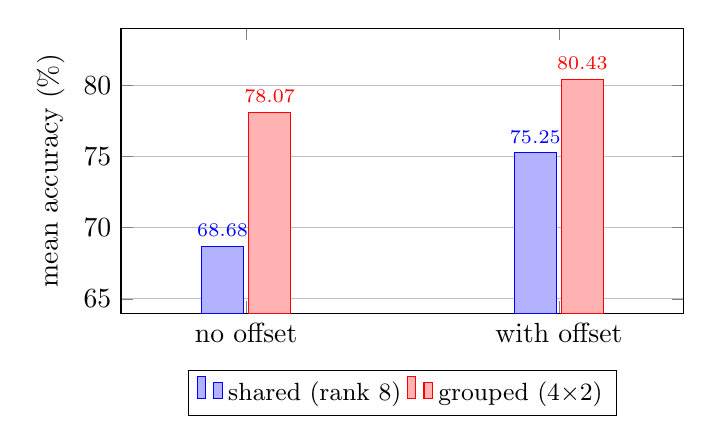
\begin{tikzpicture}
\begin{axis}[
  ybar, bar width=15pt,
  width=0.72\textwidth, height=5.2cm,
  enlarge x limits=0.4,
  ymin=64, ymax=84,
  ylabel={mean accuracy (\%)},
  symbolic x coords={no offset,with offset},
  xtick=data,
  nodes near coords, nodes near coords style={font=\scriptsize},
  legend style={at={(0.5,-0.20)},anchor=north,legend columns=2,font=\small},
  ymajorgrids, tick align=inside,
]
\addplot coordinates {(no offset,68.68) (with offset,75.25)};
\addplot coordinates {(no offset,78.07) (with offset,80.43)};
\legend{shared (rank $8$),grouped ($4{\times}2$)}
\end{axis}
\end{tikzpicture}
\caption{The two capacity moves compose at a bit-identical budget. Bars are 3-seed
mean balanced accuracy (\%) over the $12$ scorable tasks for the four corners of the
$2\times2$ (Section~\ref{sec:method}); ``with offset'' is the per-scope offset. The
proposed grouped/offset cell ($80.43$) is best on every seed, and the end-to-end
gain over the standard shared/no-offset baseline ($68.68$) is $\mathbf{+11.76}$~pp.
Family routing and the offset are scored at their upper bounds
(Section~\ref{sec:limitations}).}
\label{fig:combined-2x2}
\end{figure}

\begin{table}[t]
\centering
\small
\caption{The $2\times2$ decomposed into its four effects (3-seed means, per-seed in
brackets). Every effect is positive on all three seeds, so the two moves are
independent and additive. The grouping-alone effect here ($+9.39$~pp) is the
no-offset column of \emph{this} offset-arm run, a different arm set from the
standalone grouping experiment of Table~\ref{tab:grouping-alone} ($+8.00$~pp); both
are positive on all seeds.}
\label{tab:combined-effects}
\begin{tabular}{llc}
\toprule
effect & mean & per-seed / sign \\
\midrule
offset alone \ $(R_{\mathrm{sh{+}off}}-R_{\mathrm{sh}})$      & $+6.58$ & $+3.76,+5.29,+10.68$ \ all$+$ \\
grouping alone \ $(R_{\mathrm{gp}}-R_{\mathrm{sh}})$          & $+9.39$ & $+9.01,+8.34,+10.83$ \ all$+$ \\
grouping on top of offset \ $(R_{\mathrm{gp{+}off}}-R_{\mathrm{sh{+}off}})$ & $+5.18$ & $+6.82,+5.88,+2.84$ \ all$+$ \\
end-to-end \ $(R_{\mathrm{gp{+}off}}-R_{\mathrm{sh}})$        & $\mathbf{+11.76}$ & $+10.58,+11.18,+13.51$ \ all$+$ \\
\bottomrule
\end{tabular}
\end{table}

\noindent The proposed grouped/offset cell is best on every seed, and the two moves
are independent: grouping still adds $+5.18$~pp after the output layer is already
corrected, and the offset still adds on top of grouping, so neither subsumes the
other. The end-to-end $+11.76$~pp over the standard shared/no-offset baseline is
positive on all three seeds and roughly nine times the noise floor. This is the
paper's central positive claim: at a fixed parameter budget the two capacity
constraints of Section~\ref{sec:setup} are separately relievable and the relief adds.

\paragraph{Where the offset does \emph{not} add, stated plainly.}
The composition is not uniform across tasks, and the pattern is the expected one. The
representation gain from grouping-on-top-of-offset is concentrated on the tasks a
shared adapter had overwritten --- MNLI $+19.8$, QQP $+14.1$, RTE $+13.0$, SST-2
$+6.3$ (3-seed means of $R_{\mathrm{gp{+}off}}-R_{\mathrm{sh{+}off}}$) --- while on the
high-cardinality topic tasks the shared adapter's larger rank makes its offset-cell
competitive: DBpedia is $-0.5$ and WiC $-3.7$ under grouping. These are the same tasks
that lose in the grouping-alone breakdown and for the same reason, rank $2$ is too
small for a $14$-way label set. The net is decisively positive because the reused-token
families dominate the mean, but we report the topic-family cost rather than hide it,
and it is the concrete motivation for the adaptive per-family rank we leave to future
work.

\paragraph{Grouping de-stales the stored offset, turning its column deployable.}
The offset column above is fit against the \emph{final} model (the rehearsal ceiling
of Section~\ref{sec:sso}), an upper bound. The deployable rule fits each task's optimum
at the moment it finishes training, stores it, and never re-reads old data --- which
pays a staleness cost because the model keeps moving afterward. Section~\ref{sec:method}
argued that grouping should soften this: a family adapter is perturbed only by its own
family's later tasks, so a stored per-family optimum drifts less than one stored against
a monolithic adapter that every later task moves. We now measure it. Holding the
Chebyshev aggregation ($m{=}1$), the scope routing, and the scored \texttt{audit} split
identical, we compare the stored offset (fit at each task's boundary) against the refit
upper bound (fit against the final model); only the fit \emph{time} differs, so the gap
$\text{staleness}=R_{\mathrm{refit}}-R_{\mathrm{stored}}$ is pure staleness
(Figure~\ref{fig:destale}).

\begin{figure}[t]
\centering
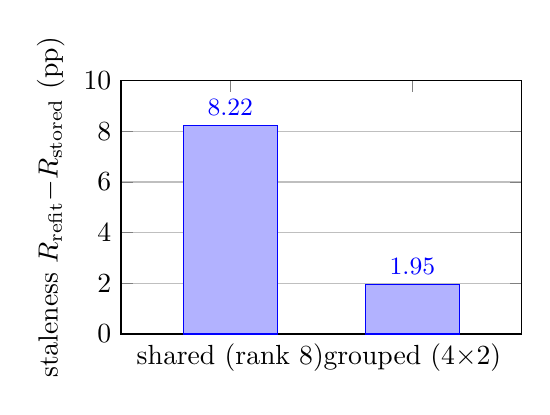
\begin{tikzpicture}
\begin{axis}[
  ybar, bar width=34pt,
  width=0.55\textwidth, height=4.8cm,
  enlarge x limits=0.6,
  ymin=0, ymax=10,
  ylabel={staleness $R_{\mathrm{refit}}{-}R_{\mathrm{stored}}$ (pp)},
  symbolic x coords={shared (rank 8),grouped ($4{\times}2$)},
  xtick=data,
  nodes near coords, nodes near coords style={font=\small},
  ymajorgrids, tick align=inside,
]
\addplot coordinates {(shared (rank 8),8.22) (grouped ($4{\times}2$),1.95)};
\end{axis}
\end{tikzpicture}
\caption{Grouping de-stales the stored offset. Bars are 3-seed mean staleness
$R_{\mathrm{refit}}-R_{\mathrm{stored}}$ (pp), holding the Chebyshev aggregation,
scope routing, and \texttt{audit} split fixed so only fit \emph{time} differs.
Grouping cuts staleness from $8.22$~pp (per-seed $7.98,10.08,6.62$) to $1.95$~pp
($1.16,3.88,0.82$): a $+6.27$~pp reduction, positive on all three seeds. The stored
offset's net gain over no offset remains mixed in sign (see text).}
\label{fig:destale}
\end{figure}

\noindent Grouping cuts the staleness of the deployable stored offset from $8.22$~pp to
$1.95$~pp, positive on all three seeds with small variance: under the grouped allocation
the deployable stored offset recovers all but $\sim2$~pp of the refit upper bound, where
on a shared adapter it forfeits over $8$~pp. This is the mechanism of
Section~\ref{sec:method} confirmed directly, and it is what lets the offset column of the
$2\times2$ be read as (near-)deployable rather than only as a ceiling. We state one
limit plainly: the stored offset's \emph{net} gain over no offset ($R_{\mathrm{stored}}-
R_{\mathrm{none}}$) is $-0.51$~pp mean under grouping and mixed in sign across seeds
($+0.14,-1.67,+0.02$), against $-1.95$~pp on the shared adapter. So grouping removes the
staleness \emph{penalty} that made the stored offset actively harmful on a shared adapter
(Section~\ref{sec:sso}'s $-5.08$~pp), but it does not, on this stream, make the deployable
offset a reliable net \emph{gain} on its own --- its value is that it now tracks the
upper-bound offset the composed method uses, closing most of the deployment gap that
Section~\ref{sec:limitations} had flagged.
